\documentclass[german,a5paper, twoside]{scrreprt} %report veraltet, scrreprt neu
%Packages
\usepackage{geometry} %Definition Satzspiegel
\geometry{left=1.5cm,right=1.5cm,top=1.5cm,bottom=1.5cm} 
\usepackage[ngerman]{babel}%auch für Umlaute???
\usepackage{bibgerm}%deutsche trennung
\usepackage[utf8]{inputenc}%Zeichensatz
\usepackage[T1]{fontenc}%fontsatz
\usepackage{geometry}
\geometry{a5paper}
\usepackage{setspace} 
\usepackage{musixtex} 
\usepackage{musixguit}
\usepackage{graphicx} %Graphiken
\usepackage{float}
\usepackage{placeins}
\usepackage{pdfpages}%mehrseitige PDFs einbinden
\usepackage{fancyhdr}%Kopfzeilen usw.
\usepackage{tikz}

\newcommand{\chort}[2]{\chord{\textbf{#1}}{#2}}
%\newcommand{\Liedname}{Fruehlingserwachen}
%\newcommand{\Abstand}{5mm}

\newcommand{\Liedname}{Fruehlingserwachen}
\newcommand{\Abstand}{4.25cm} %statt der 5cm einfach einen Abstand eingeben, damit der Text nicht mehr über den Noten ist. Faustregel: ungefähr 1.25cm pro Notenzeile

\newcommand{\Lizenz}{CC-BY-SA} %ist Standardmäßig eine CC4.0-BY-SA Lizenz. Wenn das nicht gewollt ist, CC-BY-SA einfach entfernen.



\usepackage{hyperref}

\begin{document}
\pagestyle{empty}
\begin{tikzpicture}[remember picture,overlay]
\node[anchor=north west,inner sep=5pt] at (current page.north west)
{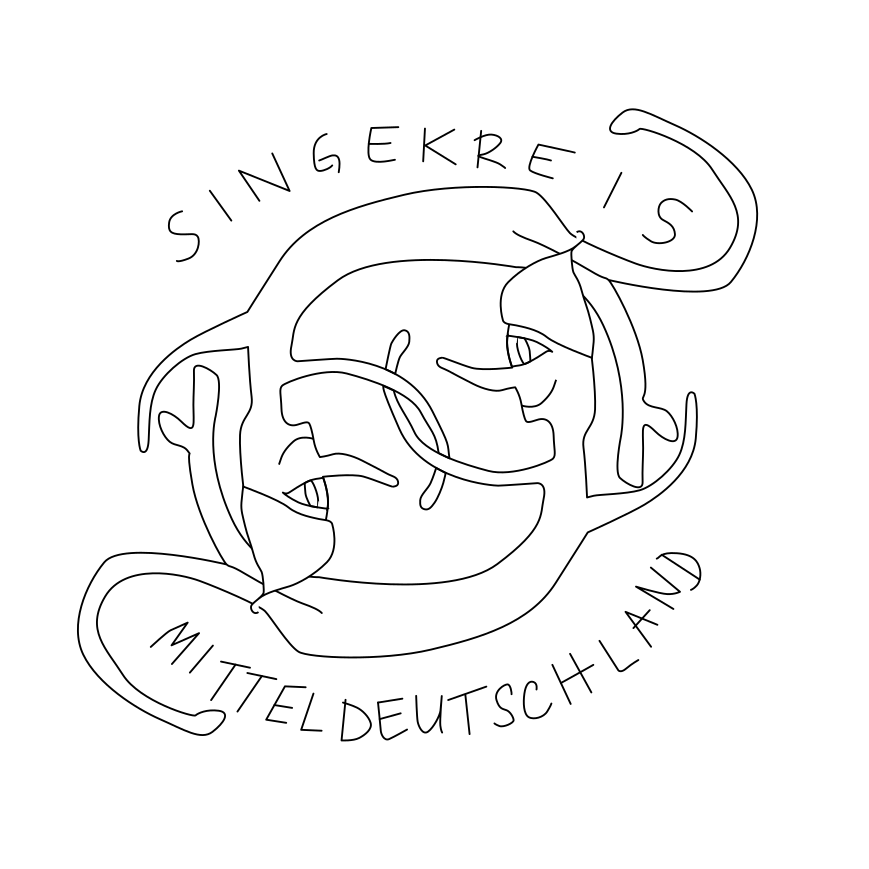
\includegraphics[width=.2\textwidth]{Rohdaten/Bilder/Singekreis.png}};
\end{tikzpicture} 
\ifthenelse{\equal{\Lizenz}{CC-BY-SA}}{
\begin{tikzpicture}[remember picture,overlay]
\node[anchor=south east,inner sep=5pt] at (current page.south east)
{
\includegraphics[width=.2\textwidth]{Rohdaten/Bilder/Lizenz.png}};
\end{tikzpicture} 
}{}
\begin{tikzpicture}[remember picture,overlay]
\node[anchor=south west,inner sep=5pt] at (current page.south west)
{
\includegraphics[width=.15\textwidth]{Rohdaten/Bilder/Schneegloeckchen.png}};
\end{tikzpicture}
\begin{tikzpicture}[remember picture,overlay]
\node[anchor=north,inner sep=10pt] at (current page.north)
{
\includegraphics[width=.4\textwidth]{Rohdaten/Bilder/ueberschrift.png}};
\end{tikzpicture}
%\vspace{-2.7cm}
%\begin{figure}[H]
%\center
%
\includegraphics[width=0.5\textwidth]{Rohdaten/Bilder/ueberschrift.png}
%\end{figure}

%\vspace{2.7cm}
\begin{figure}[t]

\includegraphics[trim=10mm 180mm 10mm 13mm, clip,width=1\textwidth]{Rohdaten/Noten/\Liedname _Noten.pdf}
\end{figure}
\vspace{-1.2cm}

\begin{song} \noindent
\textbf{2.} \chort{a}{Mo}mo \chort{C}{ruft} \chort{G}{ih}re \chort{a}{Freun}de und sie \chort{C}{tan}zen zu\chort{G}{sam}men im \chort{a}{Kreis}; \\
sie \chort{d}{stimmt} ihre \chort{C}{Fi}del und \chort{G}{je}des Kind \chort{E}{weiß}. \\
$\|$:~ Nun er\chort{a/d}{wacht} uns're \chort{C}{Mo}mo, die \chort{G}{Welt} färbt sich \chort{a}{bunt}. 
Sie \chort{(d)}{dreht} an den \chort{C}{Wir}beln und \chort{G}{spielt} eine \chort{a/E}{Rund'}. \\[0.5em]
\noindent\textbf{3.} Das \chort{a}{Sing}en mit \chort{C}{Freund}en ist \chort{G}{Le}bens\chort{a}{freu}de, musi\chort{C}{zie}ren \chort{G}{liebt} sie so \chort{a}{sehr}: \\
auf \chort{d}{Fahr}ten und \chort{C}{La}gern am \chort{G}{Berg}, auf dem \chort{E}{Meer}. \\
$\|$:~ Sie ist \chort{a/d}{wach}, uns're \chort{C}{Mo}mo, die \chort{G}{Welt} kunter\chort{a}{bunt}: 
\chort{(d)}{tan}zen, lachen \chort{C}{sing}en ist \chort{G}{al}les ge\chort{a/E}{sund}. ~:$\|$ \\[0.5em]
\noindent\textbf{4.} \chort{a}{Nacht} bricht \chort{C}{ein}, die \chort{G}{Nach}tigall \chort{a}{schlägt} und im \chort{C}{Zelt} der \chort{G}{Schlaf}sack be\chort{a}{reit}; \\
sie \chort{d}{schließt} ihre \chort{C}{Li}der und \chort{G}{dankt} für die \chort{E}{Zeit}. \\
$\|$:~ Nun \chort{a/d}{träumt} uns're \chort{C}{Mo}mo, das \chort{G}{Zelt} zittert \chort{a}{leicht}, 
\chort{(d)}{sie} schläft bis der \chort{C}{Win}ter den \chort{G}{Lenz}winden \chort{a/E}{weicht}. ~:$\|$

\noindent\textbf{Schluss:} \chort{a}{Wenn} die \chort{C}{ers}ten \chort{G}{Blü}ten sich \chort{a}{öff}nen und der \chort{E}{Wind} leise \chort{a}{weht}...

\end{song}
\begin{tikzpicture}[remember picture,overlay]
\node[anchor=south west,inner sep=5pt] at (current page.south west)
{
\includegraphics[width=.15\textwidth]{Rohdaten/Bilder/Schneegloeckchen.png}};
\end{tikzpicture}

\end{document}
